\section{Inverse Kinematik}

\textbf{Problemstellung}: siehe S. 9

Damit Inverse $\theta=f^{-1}(x)$ existiert, muss die Vorwärtskinematik $f$ bijektiv sein, aber:\\
\begin{itemize}
	\item Vorwärtskinematik ist i. A. nicht injektiv
	\begin{center}
		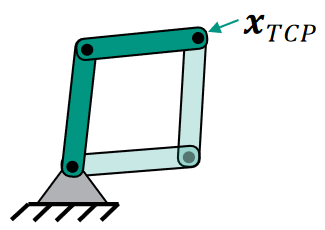
\includegraphics[width=0.2\textwidth]{images/inj.png}
	\end{center}
	\item Vorwärtskinematik ist i. A. nicht surjektiv
	\begin{center}
		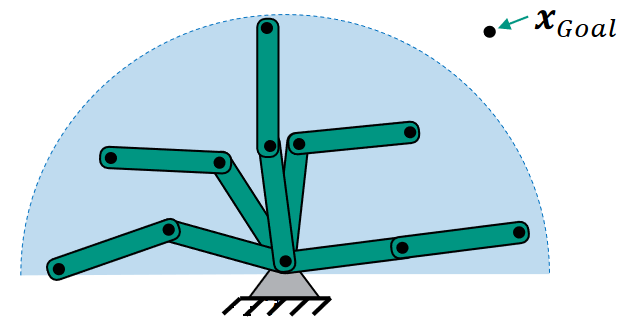
\includegraphics[width=0.3\textwidth]{images/sur.png}
	\end{center}
\end{itemize}
\bigskip
\textbf{Unterschiedliche Fälle der inversen Kinematik}:
\begin{itemize}
	\item Es gibt zwei unabhängige Lösungen (Normalfall).
	\item Es gibt genau eine Lösung (Rand des Arbeitsraums).
	\item Es gibt keine Lösung (Außerhalb des Arbeitsraums).
	\item Es gibt unendlich viele Lösungen (Zielpunkt in der Basis)
	\begin{center}
		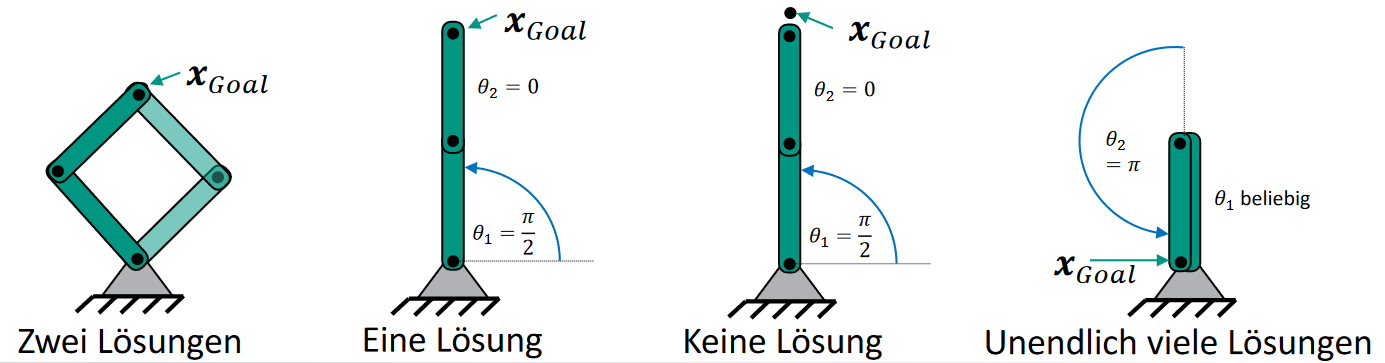
\includegraphics[width=0.8\textwidth]{images/inv-fälle.png}
	\end{center}
\end{itemize}
\bigskip
\textbf{Geometrische Methoden}:
\begin{itemize}
	\item Nutze geometrische Beziehungen (z.B. Sinus-/Kosinussatz), um $\theta$ aus $T_\text{TCP}$ zu bestimmen
	\item Bei mehreren Gelenken kann das aber sehr schwierig werden
	\item \textbf{Beispiel}: \textit{3/23-25}
\end{itemize}
\bigskip
\textbf{Algebraische Methoden}:
\begin{itemize}
	\item Führe Koeffizientenvergleich der beiden Matrizen der gewünschten TCP-Pose und der Transformation aus dem kinematischen Modell durch
	
	$\rightarrow$ 16 Gleichungen bei homogenen Matrizen, von denen 4 trivial sind (letzte Zeile immer $\irow{0 & 0 & 0 & 1}$)
	
	\item \textbf{Beispiel}: \textit{3/29-32} 
	\item \textbf{Problem}: Oft können nicht alle Gelenkwinkel aus den 12 Gleichungen bestimmt werden
	\item \textbf{Lösung}: Kenntnis der Transformationen erhöht Chance, die Gleichungen zu lösen, z.B. sei Gleichung $P_{TCP}=A_{0,1}(\theta_1)\cdot A_{1,2}(\theta_2)\cdot A_{2,3}(\theta_3)\cdot A_{3,4}(\theta_4)\cdot A_{4,5}(\theta_5)\cdot A_{5,6}(\theta_6)$ gegeben
	\begin{enumerate}
		\item Invertiere $A_{0,1}(\theta_1)$ und multipliziere beide Seiten der Gleichung mit $A_{0,1}^{-1}$
		\item Versuche im neuen Gleichungssystem den Wert einer Variablen zu bestimmen
		\item Versuche weitere Gleichung zu finden, die durch Substitution der im
		letzten Schritt gefundenen Lösung lösbar ist
		\item Falls keine Lösungen gefunden werden kann, so muss eine weitere Matrix $A_{1,2}(\theta_2)$ invertiert werden
		\item Wiederhole die Schritte 1 - 4 bis alle Gelenkwinkel ermittelt sind
	\end{enumerate}
	
	$\rightarrow$ Große Wahrscheinlichkeit, dass das Gleichungssystem gelöst werden kann
\end{itemize}
\bigskip
Im Folgenden werden \textbf{numerische Methoden} betrachtet:

\textbf{Gradientenabstieg}:
\begin{itemize}
	\item \textbf{Fehlerfunktion} für die Zielpose $\mathbf{x_\text{Goal}}\in W\colon e(\boldsymbol{\theta})=\|\mathbf{x_\text{Goal}}-f(\boldsymbol{\theta})\|^2$
	\item Wähle Startkonfiguration $\boldsymbol{\theta}_0\in C, i=0$ und Schrittlänge $\gamma\in\R$
	\item Solange $e(\boldsymbol{\theta}_i)>e_\text{Threshold}$:
	\begin{itemize}
		\item $\boldsymbol{\theta}_{i+1}=\boldsymbol{\theta}_i-\gamma\cdot 2\cdot J^T(\boldsymbol{\theta}_i)\cdot(f(\boldsymbol{\theta}_i)-\mathbf{x_\text{Goal}})$, wobei $J$ die Jacobi-Matrix der Vorwärtskinematik ist
		\item $i=i+1$
	\end{itemize}
	\item Je nach gewählter Startkonfiguration erhält man unterschiedliche Lösungen
\end{itemize}
\bigskip
\textbf{Pseudoinverse}:
\begin{itemize}
	\item \textbf{Differenzenquotient}: 
	\begin{itemize}
		\item Tatsächliche Bewegung gemäß $\mathbf{\dot{x}}(t)=J(\boldsymbol{\theta}(t))\cdot\boldsymbol{\dot{\theta}}(t)$
		\item Annäherung mittels Differenzenquotient: $\Delta\mathbf{x}\approx J(\boldsymbol{\theta})\Delta\boldsymbol{\theta}$
	\end{itemize}
	\begin{center}
		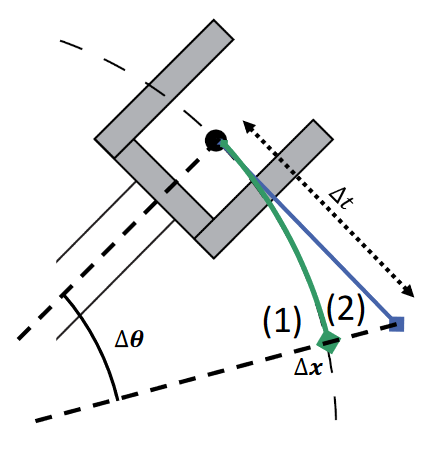
\includegraphics[width=0.3\textwidth]{images/dq.png}
	\end{center}
	\item Suche Lösung für das inverse Problem: $\Delta\boldsymbol{\theta}=J_f^{-1}(\boldsymbol{\theta})\cdot\Delta\mathbf{x}$, aber $J_f$ muss nicht unbedingt invertierbar sein $\rightarrow$ Nutze Pseudoinverse
	\item Es lässt sich herleiten: $$\Delta\boldsymbol{\theta}=(J_f^\top J_f)^{-1}J_f^\top \Delta\mathbf{x}=J_f^+(\boldsymbol{\theta})\Delta\mathbf{x}$$
	wobei $J_f^+$ die \textbf{Pseudoinverse} von $J_f$ ist ($A^+=(A^\top A)^{-1}A^\top$)
	\item \textbf{Algorithmus}:
	\begin{center}
		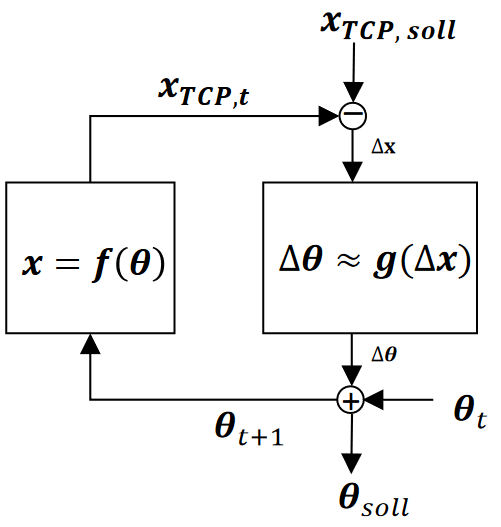
\includegraphics[width=0.3\textwidth]{images/pseudoinverse.png}
	\end{center}
	\item \textbf{Problem}: Pseudoinverse ist in der Nähe von Singularitäten instabil!
	\item \textbf{Lösung}: \textbf{Damped least squares}-Methode
\end{itemize}

\textbf{Damped Least Squares}:
\begin{itemize}
	\item Führe Dämpfungskonstante $\lambda>0$ ein und berechne 
	$$\Delta\boldsymbol{\theta}=J^\top(JJ^\top+\lambda^2I)^{-1}\Delta\mathbf{x}$$
	\item Analyse der Stabilität über \textbf{Singulärwertzerlegung}: $J=UDV^T=\sum\limits_{i=1}^r \sigma_i \mathbf{u_iv_i^\top}$, wobei $U,V$ orthogonale Matrizen, $D$ Diagonalmatrix mit Singulärwerten auf der Diagonalen, $\mathbf{u_i},\mathbf{v_i}$ die $i$-te Spalte von $U$ bzw. $V$ und $r$ der rang von $J$ ist
	\newpage
	
	\item Es lässt sich herleiten:
	\begin{itemize}
		\item Pseudoinverse: $J^+=\sum\limits_{i=1}^r \frac{1}{\sigma_i}\mathbf{v_i} \mathbf{u_i}^\top$
		\item Damped Least Squares: $J^\top(JJ^\top+\lambda^2I)^{-1}=\sum\limits_{i=1}^r \frac{\sigma_i}{\sigma_i^2+\lambda^2}\mathbf{v_i}\mathbf{u_i^\top}$
		
		$\rightarrow$ Für $\sigma_i\rightarrow 0$ wird die Pseudoinverse instabil, Damped-Least-Squares bleibt aber wohldefiniert. Für große $\sigma_i$ verglichen mit $\lambda$ verhält sich Damped-Least-Squares wie die Pseudoinverse.
	\end{itemize}
\end{itemize}